\documentclass[12pt, oneside, titlepage]{article}   	% use "amsart" instead of "article" for AMSLaTeX format
\usepackage{geometry}                     
\usepackage{amsmath}                      
\usepackage{amssymb}                       
\usepackage{bm}   
\usepackage{tabularx}   
\usepackage{caption}          
 \captionsetup[table]{labelfont=sc}

\usepackage{booktabs}

\usepackage{graphicx}

\usepackage{rotating}


%%%%%%%%%%%%%%%%%%%%%%%%%%%%%%%%%%%%%%%%%%%%%%%%%%%%
%%%%%%%%%%%%%%%%%%%%%%%%%%%%%%%%%%%%%%%%%%%%%%%%%%%%
% begin document
%%%%%%%%%%%%%%%%%%%%%%%%%%%%%%%%%%%%%%%%%%%%%%%%%%%%
%%%%%%%%%%%%%%%%%%%%%%%%%%%%%%%%%%%%%%%%%%%%%%%%%%%%

\begin{document}

%%%%%%%%%%%%%%%%%%%%%%%%%%%%%%%%%%
% DATASETS
%%%%%%%%%%%%%%%%%%%%%%%%%%%%%%%%%%

\begin{center}
\captionof{table}{ Summary of data sets used to estimate parameters. } \label{tab:title1} 
 \begin{tabularx}{\linewidth}{ l l c c } 
 \hline
 \hline
\multicolumn{1}{ c }{ Parameter data } & 
\multicolumn{1}{ c }{ Description } & 
\multicolumn{1}{ c }{ Data set }  & 
\multicolumn{1}{ c }{ Time span } \\
 \hline
 % seed bag burial experiment
 \textsc{Seed vital rates} & --- & --- & --- \\ 
 Seed survival and germination & Seed bag burial & $\bm{\mathrm{Y}}_1$ & 2006-2009  \\ 
 Seed viability & Viability trials & $\bm{\mathrm{Y}}_2$ & 2006-2009 \\ 
 Seed survival and germination & Seed pots & $\bm{\mathrm{Y}}_3$ & 2013-2019  \\ 
 \textsc{Seedling survival} & --- & --- & --- \\ 
 Seedling survival to fruiting & Field surveys & $\bm{\mathrm{Y}}_4$ & 2006-2019 \\ 
 \textsc{Fruits per plant} & --- & --- & --- \\ 
 Total fruit equivalents per plant & Field surveys & $\bm{\mathrm{Y}}_5$ & 2006-2012 \\ 
 Undamaged and damaged fruits per plant & Field surveys & $\bm{\mathrm{Y}}_6$ & 2013-2019 \\ 
 Total fruit equivalents per plant & Extra plots & $\bm{\mathrm{Y}}_7$ & 2006-2012 \\ 
 Undamaged and damaged fruits per plant & Extra plots & $\bm{\mathrm{Y}}_8$ & 2013-2019 \\ 
 \textsc{Seeds per fruit} & --- & --- & --- \\ 
  Seeds per undamaged fruit & Lab counts & $\bm{\mathrm{Y}}_9$ & 2006-2019 \\ 
  Seeds per damaged fruit & Lab counts & $\bm{\mathrm{Y}}_{10}$ & 2013-2019 \\   
  \hline
\end{tabularx}
\end{center}

\newpage

%%%%%%%%%%%%%%%%%%%%%%%%%%%%%%%%%%
% PARAMETERS
%%%%%%%%%%%%%%%%%%%%%%%%%%%%%%%%%%

\begin{center}
\captionof{table}{ Description of key parameters. } \label{tab:title2} 
 \begin{tabularx}{\linewidth}{c X} 
 \hline
 \hline
\multicolumn{1}{ c }{ Parameter } & 
\multicolumn{1}{ c }{ Description } \\
 \hline
 % seed bag burial experiment
 $\theta_1$ & Probability of survival of seeds from October in year $t$ to January in year $t+1$, for seeds produced in year $t$ \\ 

 $\theta_2$ & Probability of emergence of seeds in January in year $t+1$, conditional on being intact or a germinant in January in year $t+1$, for seeds produced in year $t$ \\
 
 $\theta_3$ & Probability of survival of seeds from January in year $t+1$ to October in year $t+1$, conditional on being intact in January in year $t+1$, for seeds produced in year $t$  \\
 
 $\theta_4$ & Probability of survival of seeds from October in year $t$ to January in year $t+2$, for seeds produced in year $t$ \\
  
 $\theta_5$ & Probability of emergence of seeds in January in year $t+2$, conditional on being intact or a germinant in January in year $t+2$, for seeds produced in year $t$  \\
 
 $\nu_1$ & Probability of viability for seeds in October of year $t+1$, for seeds produced in year $t$ \\
 
 $\nu_2$ & Probability of survival for seeds in October of year $t+2$, for seeds produced in year $t$ \\

 $\sigma$ & Probability of survival of seedlings to fruiting plants\\

 $F$ & Number of total fruit equivalents per plant \\
 
 $\phi$ & Number of seeds per undamaged fruit \\ 
  \hline
\end{tabularx}
\end{center}

\newpage



%%%%%%%%%%%%%%%%%%%%%%%%%%%%%%%%%%
% SEED BAG BURIAL EXPERIMENT
%%%%%%%%%%%%%%%%%%%%%%%%%%%%%%%%%%

\captionof{table}{ Summary of dataset from seed bag burial experiment. [Data set $\bm{\mathrm{Y}}_1$]  } \label{tab:titleburial} 
\begin{table}[ht]
\centering
\begin{tabular}{lcccccc}
  \hline
  \hline
 &  \multicolumn{3}{c}{Age 1} & \multicolumn{2}{c}{Age 2} & Age 3 \\
 \cmidrule(lr){2-4} \cmidrule(lr){5-6} \cmidrule(lr){7-7} 
Population & 2007 & 2008 & 2009 & 2008 & 2009 & 2009 \\ 
  \hline
BG &   7 &  10 &  10 &   6 &  10 &   3 \\ 
  BR &  10 &  10 &  10 &   9 &  10 &   9 \\ 
  CF &  10 &  10 &  10 &  10 &  10 &  10 \\ 
  CP3 &   7 &  10 &   8 &   9 &   5 &   7 \\ 
  DEM &   8 &   9 &  10 &   7 &   7 &   6 \\ 
  DLW &   9 &   9 &   8 &   8 &   9 &   6 \\ 
  EC &   9 &   9 &  10 &   8 &  10 &   8 \\ 
  FR &   9 &   7 &  10 &   8 &   9 &   3 \\ 
  GCN &  10 &  10 &  10 &   9 &   9 &   6 \\ 
  KYE &  10 &  10 &  10 &   9 &   9 &   9 \\ 
  LCE &  10 &  10 &   9 &   9 &   7 &   7 \\ 
  LCW &  10 &  10 &   5 &   9 &   7 &   8 \\ 
  LO &  10 &   9 &  10 &  10 &  11 &   9 \\ 
  MC &  10 &  10 &  10 &   8 &   9 &   9 \\ 
  OKRE &  10 &  11 &  10 &   9 &   7 &   9 \\ 
  OKRW &  10 &  10 &   8 &   9 &   9 &   7 \\ 
  OSR &  10 &  10 &  10 &   8 &   9 &   9 \\ 
  S22 &   9 &  10 &  10 &   8 &  10 &   8 \\ 
  SM &   9 &  10 &   9 &   8 &  10 &   9 \\ 
  URS &   7 &   9 &   9 &   5 &   9 &   3 \\ 
   \hline
\end{tabular}
\end{table}
 
 \newpage
 
%%%%%%%%%%%%%%%%%%%%%%%%%%%%%%%%%%
% VIABILITY FOR SEED BAG BURIAL EXPERIMENT
%%%%%%%%%%%%%%%%%%%%%%%%%%%%%%%%%%

\captionof{table}{ Summary of dataset on viability of seeds from seed bag burial experiment. [Data set $\bm{\mathrm{Y}}_2$] } \label{tab:titleviab} 
\begin{table}[ht]
\centering
\begin{tabular}{lcccccc}
  \hline
  \hline
 &  \multicolumn{3}{c}{Age 1} & \multicolumn{2}{c}{Age 2} & Age 3 \\
 \cmidrule(lr){2-4} \cmidrule(lr){5-6} \cmidrule(lr){7-7} 
Population & 2007 & 2008 & 2009 & 2008 & 2009 & 2009 \\ 
  \hline
BG &   7 &  10 &  10 &   6 &  10 &   3 \\ 
  BR &  10 &   9 &  10 &  10 &  10 &   9 \\ 
  CF &  10 &  10 &  10 &   9 &  10 &  10 \\ 
  CP3 &   7 &  10 &   9 &   8 &   7 &   7 \\ 
  DEM &   8 &   9 &  10 &   6 &   7 &   5 \\ 
  DLW &   8 &   9 &   9 &   8 &   9 &   7 \\ 
  EC &   9 &  10 &  10 &   8 &  10 &   6 \\ 
  FR &   8 &   8 &  10 &   8 &  10 &   4 \\ 
  GCN &   9 &  10 &  10 &   8 &   9 &   7 \\ 
  KYE &  10 &  10 &  10 &   9 &   9 &   9 \\ 
  LCE &  10 &  10 &   9 &   9 &   6 &   9 \\ 
  LCW &  10 &  10 &   5 &   9 &   7 &   7 \\ 
  LO &  11 &   9 &  10 &   9 &  10 &   9 \\ 
  MC &   9 &   9 &  10 &   8 &   9 &   9 \\ 
  OKRE &  10 &  11 &  10 &   9 &   7 &   9 \\ 
  OKRW &   9 &  10 &   8 &   8 &   9 &   7 \\ 
  OSR &  10 &  10 &  10 &   8 &   9 &   9 \\ 
  S22 &   9 &  10 &  10 &   8 &  10 &   8 \\ 
  SM &   8 &  10 &   9 &   8 &  10 &  11 \\ 
  URS &   7 &   9 &   9 &   5 &   8 &   4 \\ 
   \hline
\end{tabular}
\end{table}

 \newpage
 
%%%%%%%%%%%%%%%%%%%%%%%%%%%%%%%%%%
% SEEDLING SURVIVAL TO FRUITING
%%%%%%%%%%%%%%%%%%%%%%%%%%%%%%%%%%

 \small
% Let LaTeX figure out amount of intercolumn whitespace
\setlength\tabcolsep{0pt} 


\captionof{table}{ Summary of dataset on seedling survival to fruiting. [Data set $\bm{\mathrm{Y}}_4$] } \label{tab:sigma} 
\
\centering
\begin{tabular*}{\textwidth}{ l @{\extracolsep{\fill}} *{26}{c} }
  \hline
  \hline
  Population & 2006 & 2007 & 2008 & 2009 & 2010 & 2011 & 2012 & 2013 & 2014 & 2015 & 2016 & 2017 \\ 
  \hline
BG &  18 &  21 &  22 &  26 &  24 &  26 &  20 &  23 &   3 &  26 &   5 &  16 \\ 
  BR &  19 &  30 &  29 &  30 &  30 &  30 &  29 &  30 &   9 &  27 &   5 &  26 \\ 
  CF &  20 &  21 &  28 &  29 &  29 &  21 &  23 &  27 &  15 &  15 &   5 &  22 \\ 
  CP3 &  18 &  19 &  19 &  13 &  19 &   8 & -- &  10 &   1 &   7 & -- &   6 \\ 
  DEM &  18 &  17 &  14 &  21 &  24 &  25 &  18 &  22 &   3 &   9 &   4 &  21 \\ 
  DLW &  16 &  18 &  13 &  15 &  17 &  22 &  16 &  19 &   1 &  13 &   5 &  11 \\ 
  EC &  20 &  28 &  30 &  30 &  30 &  30 &  30 &  24 &   2 &  10 &   9 &   8 \\ 
  FR &  20 &  28 &  27 &  27 &  30 &  30 &  24 &  25 &   7 &  15 &   3 &  17 \\ 
  GCN &  18 &  20 &  15 &  20 &  28 &  29 &  22 &  27 &   5 &  17 & -- &   1 \\ 
  KYE &  18 &  28 &  28 &  30 &  30 &  30 &  27 &  28 &   1 &  27 &   9 &  12 \\ 
  LCE &  20 &  12 &  18 &  19 &  19 &   1 &   1 &   3 &   1 &   8 &   7 &  19 \\ 
  LCW &  16 &  27 &  27 &  27 &  21 &   4 & -- &  15 & -- &   1 & -- &   4 \\ 
  LO &  12 &  15 &  28 &  29 &  27 &   2 &   1 &  19 &   5 &  11 &   6 &  19 \\ 
  MC &  17 &  11 &  22 &  25 &  27 &  30 &  29 &  27 &   6 &  18 &   8 &  15 \\ 
  OKRE &  14 &  10 &   8 &  19 &  21 &  17 &   7 &  19 &   6 &  10 &   5 &  15 \\ 
  OKRW &  19 &  19 &  22 &  20 &  19 &  12 &   9 &  13 & -- &   3 &   1 &   3 \\ 
  OSR &  15 &  13 &   9 &   9 &  23 &  26 &  18 &  20 &   1 &  14 & -- &   1 \\ 
  S22 &  17 &  10 &  21 &  18 &  28 &  17 &  27 &  26 & -- &  17 &   4 &  10 \\ 
  SM &  15 &   8 &  13 &  18 &  23 &  25 &  18 &  24 & -- &  19 &   8 &  13 \\ 
  URS &   4 &  17 &  10 &   7 &  12 &  14 &   3 &   5 &   2 &   1 & -- &   5 \\ 
   \hline
\end{tabular*}


\newpage

%%%%%%%%%%%%%%%%%%%%%%%%%%%%%%%%%%
% UNDERCOUNTING FOR SEEDLING SURVIVAL TO FRUITING
%%%%%%%%%%%%%%%%%%%%%%%%%%%%%%%%%%

 \captionof{table}{ Summary of undercounting in the dataset on seedling survival to fruiting. Values are the percentage of plots with more fruiting plants than seedlings. } \label{tab:undercount} 
\centering
\
\begin{tabular*}{\textwidth}{ l @{\extracolsep{\fill}} *{26}{c} }
  \hline
  \hline
Population & 2006 & 2007 & 2008 & 2009 & 2010 & 2011 & 2012 & 2013 & 2014 & 2015 & 2016 & 2017 \\ 
  \hline
BG & 0.00 & 14.00 & 9.10 & 0.00 & 12.00 & 0.00 & 5.00 & 0.00 & 0.00 & 0.00 & 0.00 & 0.00 \\ 
  BR & 0.00 & 3.30 & 10.00 & 0.00 & 33.00 & 0.00 & 3.40 & 0.00 & 44.00 & 0.00 & 20.00 & 0.00 \\ 
  CF & 0.00 & 9.50 & 7.10 & 3.40 & 17.00 & 9.50 & 0.00 & 0.00 & 6.70 & 0.00 & 0.00 & 4.50 \\ 
  CP3 & 0.00 & 5.30 & 21.00 & 15.00 & 0.00 & 12.00 & -- & 0.00 & -- & 0.00 & -- & 0.00 \\ 
  DEM & 0.00 & 35.00 & 14.00 & 0.00 & 29.00 & 4.00 & 0.00 & 0.00 & 0.00 & 0.00 & 0.00 & 0.00 \\ 
  DLW & 0.00 & 11.00 & 7.70 & 13.00 & 29.00 & 4.50 & 6.20 & 0.00 & 0.00 & 0.00 & 40.00 & 0.00 \\ 
  EC & 0.00 & 29.00 & 30.00 & 0.00 & 20.00 & 0.00 & 0.00 & 21.00 & 50.00 & 0.00 & 11.00 & 0.00 \\ 
  FR & 5.00 & 3.60 & 7.40 & 3.70 & 0.00 & 0.00 & 0.00 & 0.00 & 43.00 & 0.00 & 33.00 & 0.00 \\ 
  GCN & 0.00 & 0.00 & 27.00 & 0.00 & 29.00 & 17.00 & 0.00 & 0.00 & -- & 0.00 & -- & 0.00 \\ 
  KYE & 0.00 & 3.60 & 29.00 & 0.00 & 47.00 & 3.30 & 0.00 & 3.60 & -- & 3.70 & 0.00 & 0.00 \\ 
  LCE & 0.00 & 50.00 & 5.60 & 37.00 & 5.30 & 0.00 & 0.00 & 0.00 & 0.00 & 0.00 & 14.00 & 5.30 \\ 
  LCW & 0.00 & 3.70 & 0.00 & 0.00 & 4.80 & 25.00 & -- & 0.00 & -- & 0.00 & -- & 0.00 \\ 
  LO & 0.00 & 33.00 & 7.10 & 6.90 & 0.00 & -- & 0.00 & 0.00 & 0.00 & 9.10 & 33.00 & 11.00 \\ 
  MC & 0.00 & 27.00 & 4.50 & 8.00 & 7.40 & 0.00 & 0.00 & 0.00 & 33.00 & 0.00 & 38.00 & 6.70 \\ 
  OKRE & 0.00 & 20.00 & 12.00 & 11.00 & 14.00 & 18.00 & 0.00 & 0.00 & 17.00 & 0.00 & 20.00 & 6.70 \\ 
  OKRW & 0.00 & 5.30 & 0.00 & 5.00 & 37.00 & 33.00 & 0.00 & 0.00 & -- & 0.00 & -- & 0.00 \\ 
  OSR & 0.00 & 7.70 & 11.00 & 0.00 & 39.00 & 15.00 & 0.00 & 0.00 & -- & 0.00 & -- & 0.00 \\ 
  S22 & 0.00 & 0.00 & 19.00 & 5.60 & 18.00 & 18.00 & 3.70 & 0.00 & -- & 0.00 & 50.00 & 0.00 \\ 
  SM & 0.00 & 0.00 & 23.00 & 0.00 & 61.00 & 20.00 & 0.00 & 4.20 & -- & 0.00 & 0.00 & 0.00 \\ 
  URS & 0.00 & 5.90 & 0.00 & 14.00 & 17.00 & 7.10 & 0.00 & 0.00 & 0.00 & 0.00 & -- & 0.00 \\ 
      \hline
\end{tabular*}

\clearpage

\normalsize

% return to default
 \setlength\tabcolsep{6pt} 

\iffalse
 
  \begin{figure}[h]
   \centering
       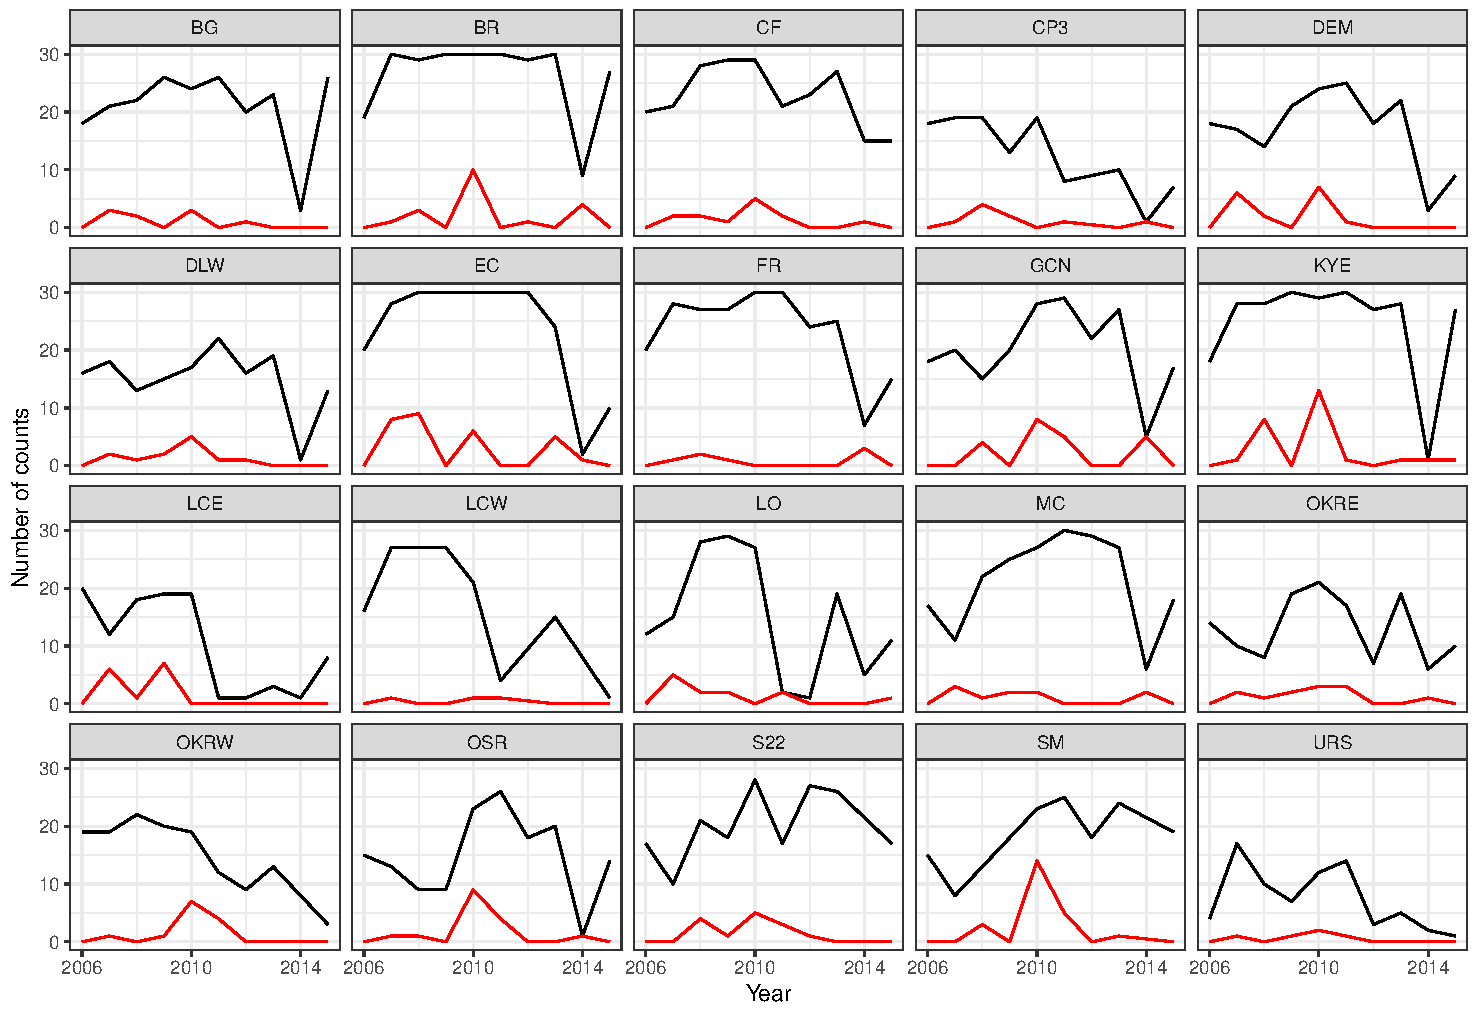
\includegraphics[width=\textwidth]{/Users/gregor/Dropbox/clarkiaSeedBanks/products/figures/underCounting.pdf}  
    \caption{ Graphical summary of undercounting in the dataset on seedling survival to fruiting. Each panel summarizes the datasets on seedling survival to fruiting (Tables~\ref{tab:sigma} and~\ref{tab:undercount}). The black lines correspond to total plots with data on seedling survival. The red lines correspond to the number of plots with fewer seedlings than fruiting plants in a plot (corresponding to undercounting). }
 \label{fig:obs_pred}
\end{figure}

\fi
 
   \clearpage
   
%%%%%%%%%%%%%%%%%%%%%%%%%%%%%%%%%%
% FRUITS PER PLANT: TOTAL FRUIT EQUIVALENTS FROM PLOTS
%%%%%%%%%%%%%%%%%%%%%%%%%%%%%%%%%%
  
\captionof{table}{ Summary of dataset on total fruit equivalents per plant from transects. [Data set $\bm{\mathrm{Y}}_5$] } \label{tab:sigma} 
\begin{table}[ht]
\centering
\begin{tabular}{lcccccc}
  \hline
Population & 2007 & 2008 & 2009 & 2010 & 2011 & 2012 \\ 
  \hline
BG &  42 & 145 &  47 & 151 & 105 &  11 \\ 
  BR & 172 & 515 & 222 & 377 & 153 &  61 \\ 
  CF &  22 &  75 & 118 & 321 & 164 &  29 \\ 
  CP3 &  29 &  18 &  23 &  23 &   4 & -- \\ 
  DEM &  70 &  56 & 139 & 200 & 100 &  15 \\ 
  DLW &   6 &   8 &  11 &  40 &  34 &  19 \\ 
  EC & 122 & 126 & 253 & 350 & 289 &  25 \\ 
  FR & 100 &  21 & 115 & 326 &  94 &   3 \\ 
  GCN & -- &   8 & -- & 107 & 179 &  17 \\ 
  KYE &  40 & 151 & 112 & 251 & 195 &   3 \\ 
  LCE &  25 &  66 &  41 &   6 & -- & -- \\ 
  LCW & 253 & 266 &  16 &  58 &   3 & -- \\ 
  LO &  15 & 187 & 472 &  68 &   2 &   1 \\ 
  MC &  24 &  33 &  56 & 150 & 188 &   4 \\ 
  OKRE &  11 &  11 &  27 &  57 &  35 &   1 \\ 
  OKRW &   8 &  14 &  24 & 103 &  10 & -- \\ 
  OSR &  13 &  20 &  36 & 159 & 129 &  32 \\ 
  S22 & -- &  23 &  30 & 102 &  22 &   3 \\ 
  SM &   5 &  26 &  42 & 137 & 159 &   2 \\ 
  URS &   3 &   3 &   2 &  10 &  17 &   1 \\ 
   \hline
\end{tabular}
\end{table}

 \newpage
 
%%%%%%%%%%%%%%%%%%%%%%%%%%%%%%%%%%
% FRUITS PER PLANT: UNDAMAGED/DAMAGED FRUITS PER PLANT FROM PLOTS
%%%%%%%%%%%%%%%%%%%%%%%%%%%%%%%%%%
 
 \captionof{table}{   Summary of dataset on undamaged and damaged fruits per plant from transects. [Data set $\bm{\mathrm{Y}}_6$] } \label{tab:sigma} 
\begin{table}[ht]
\centering
\begin{tabular}{lcccccc}
  \hline
Population & 2013 & 2014 & 2015 & 2016 & 2017 & 2018 \\ 
  \hline
BG &   7 &   3 & -- &   3 &  12 &  38 \\ 
  BR &  32 &   8 &   3 &   5 &  46 & 107 \\ 
  CF &  13 &  12 &   2 &   6 &  33 & -- \\ 
  CP3 &   2 &   1 & -- & -- &   1 & -- \\ 
  DEM &  12 &   3 &   2 &   5 & 134 & 156 \\ 
  DLW &   2 & -- & -- &   4 &  11 &  11 \\ 
  EC &  13 &   1 &  15 &   2 &   9 & -- \\ 
  FR & -- &   4 &   1 &   1 &  42 &  13 \\ 
  GCN &   1 &   9 &   3 & -- & -- &   4 \\ 
  KYE &   6 &   1 &  19 & -- &   3 &   4 \\ 
  LCE & -- & -- &   1 &  14 &  24 &  73 \\ 
  LCW & -- & -- & -- & -- & -- &   1 \\ 
  LO &   6 &   2 &   1 &   6 &  12 &  11 \\ 
  MC & -- &   3 & -- &   7 &  10 & -- \\ 
  OKRE &   5 &   3 &   1 &   2 &  19 &   4 \\ 
  OKRW & -- & -- & -- &   1 &   4 &   1 \\ 
  OSR &   1 &   1 & -- & -- & -- & -- \\ 
  S22 &   1 & -- &   4 &   4 &   6 & -- \\ 
  SM &   8 & -- &   9 & -- & -- & -- \\ 
  URS & -- & -- & -- & -- &   3 & -- \\ 
     \hline
\end{tabular}
\end{table}

  \newpage
  
%%%%%%%%%%%%%%%%%%%%%%%%%%%%%%%%%%
% FRUITS PER PLANT: TOTAL FRUIT EQUIVALENTS EXTRA PLOTS
%%%%%%%%%%%%%%%%%%%%%%%%%%%%%%%%%%
  
\captionof{table}{ Summary of dataset on total fruit equivalents per plant from extra plots. [Data set $\bm{\mathrm{Y}}_7$] } \label{tab:sigma} 
\begin{table}[ht]
\centering
\begin{tabular}{lccccccc}
  \hline
Population & 2006 & 2007 & 2008 & 2009 & 2010 & 2011 & 2012 \\ 
  \hline
BG & 153 & 118 &  77 & 108 & -- &  38 &  52 \\ 
  BR & 349 &  58 & 229 &  17 & 115 &  48 &  64 \\ 
  CF & 282 & 143 & 150 &  68 &  38 &  74 &  68 \\ 
  CP3 & 279 & 197 & 128 & 178 & 177 & 103 &  25 \\ 
  DEM & 177 &  67 & -- &  52 & 188 &  28 &  78 \\ 
  DLW & 208 & 124 & 110 & 139 & 147 &  70 &  54 \\ 
  EC & 370 &  74 &   7 &  34 &  46 & 112 &  58 \\ 
  FR & 261 &  88 & 133 &  61 & 102 &  57 &  14 \\ 
  GCN & 240 & 169 & 148 & 125 & 161 &  79 & 136 \\ 
  KYE & 285 & 155 & 174 &  87 & 155 &  30 &  72 \\ 
  LCE & 246 & 194 &  81 & 105 & 127 &  29 &   0 \\ 
  LCW & 243 &  17 &  75 & 178 & 167 &  50 &   3 \\ 
  LO &  98 &  98 &  67 & -- & 132 &  38 &   2 \\ 
  MC & 163 & 133 & 109 &  95 &  56 &  90 &  73 \\ 
  OKRE & 100 &  36 &  32 & 113 &  50 &  87 &   4 \\ 
  OKRW & 280 &  52 &  57 &  51 & 125 &  91 &   6 \\ 
  OSR & 277 & 288 & 246 & 150 & 157 & 145 & 117 \\ 
  S22 & 319 & 111 &  69 & 157 & 144 &  83 & 112 \\ 
  SM & 217 &  20 &  53 &  79 &  33 &  41 &  49 \\ 
  URS &  32 &  40 &  38 &  52 & 145 &  40 &   6 \\ 
   \hline
\end{tabular}
\end{table}

  \newpage
 
 %%%%%%%%%%%%%%%%%%%%%%%%%%%%%%%%%%
% FRUITS PER PLANT: UNDAMAGED/DAMAGED FRUITS EXTRA PLOTS
%%%%%%%%%%%%%%%%%%%%%%%%%%%%%%%%%%
 
 \captionof{table}{   Summary of dataset on undamaged and damaged fruits per plant from extra plots. [Data set $\bm{\mathrm{Y}}_9$] } \label{tab:sigma} 
\begin{table}[ht]
\centering
\begin{tabular}{lcccccc}
  \hline
Population & 2013 & 2014 & 2015 & 2016 & 2017 & 2018 \\ 
  \hline
BG &  34 &  89 &  52 &  53 &  90 & 126 \\ 
  BR &  82 & 173 &  62 &  79 & 134 & 167 \\ 
  CF &  58 & 102 &  50 &  90 & 165 & 150 \\ 
  CP3 & 149 &  87 &  59 &  69 & 141 &  11 \\ 
  DEM &  20 &  43 &  43 &  62 & 121 & 100 \\ 
  DLW &  66 &  35 &  61 &  56 & 232 & 158 \\ 
  EC &  41 &  41 &  81 &  64 & 142 &   6 \\ 
  FR &   6 &  55 &  40 &  52 & 156 &  61 \\ 
  GCN &   9 &  35 &  55 &  64 & 103 & 130 \\ 
  KYE &  54 & 135 & 101 &  57 & 141 & 129 \\ 
  LCE &  25 &  53 &  60 & 135 &  94 &  82 \\ 
  LCW &   0 &   0 &   0 &   0 &  48 & 154 \\ 
  LO &   2 &  46 & -- &   8 & 175 &  38 \\ 
  MC &   5 &  74 &  44 &  46 & 122 & 113 \\ 
  OKRE &  63 &  28 &  31 &  38 &  78 &  32 \\ 
  OKRW &   0 &   8 &   0 &  31 & 126 &  34 \\ 
  OSR &  46 & 159 & 104 &  99 & 150 & 108 \\ 
  S22 & -- &  29 &  65 & 102 & 253 &  18 \\ 
  SM &  52 &   3 &  19 &   0 &  53 &  18 \\ 
  URS &   0 &   0 &   0 &  79 &  35 &   0 \\ 
     \hline
\end{tabular}
\end{table}
 
\newpage

%%%%%%%%%%%%%%%%%%%%%%%%%%%%%%%%%%
% SEEDS PER UNDAMAGED FRUIT
%%%%%%%%%%%%%%%%%%%%%%%%%%%%%%%%%%

 \small
% Let LaTeX figure out amount of intercolumn whitespace
\setlength\tabcolsep{0pt} 


\captionof{table}{ Summary of dataset on seeds per undamaged fruit. [Data set $\bm{\mathrm{Y}}_9$] } \label{tab:titleviab} 
\centering
\begin{tabular*}{\textwidth}{ l @{\extracolsep{\fill}} *{26}{c} }
  \hline
  \hline
Population & 2006 & 2007 & 2008 & 2009 & 2010 & 2011 & 2012 & 2013 & 2014 & 2015 & 2016 & 2017 & 2018 \\ 
  \hline
BG &  21 &  19 &  41 &  30 &  30 &  28 &  29 &  29 &  30 &  29 &  29 &  32 &  27 \\ 
  BR &  20 &  29 &  32 &  30 &  29 &  18 &  29 &  39 &  31 &  31 &  30 &  27 &  32 \\ 
  CF &  20 &  45 &  30 &  29 &  34 &  30 &  27 &  28 &  30 &  26 &  28 &  31 &  33 \\ 
  CP3 &  20 &  36 &  41 &  30 &  30 &  29 &  21 &  30 &  30 &  21 &  29 &  29 &  11 \\ 
  DEM &  20 &  32 &  29 &  30 &  32 &  27 &  27 &  30 &  24 &  28 &  30 &  25 &  29 \\ 
  DLW &  20 &  29 &  22 &  30 &  31 &  28 &  25 &  33 &   1 &  30 &  29 &  32 &  35 \\ 
  EC &  20 &  17 &  29 &  30 &  31 &  26 &  22 &  30 &  31 &  31 &  30 &  30 &   4 \\ 
  FR &  20 &  34 &  31 &  30 &  31 &  31 &  10 &   2 &  46 &  30 &  38 &  31 &  31 \\ 
  GCN &  20 &  29 &  29 &  30 &  32 &  30 &  29 &  27 &  28 &  29 &  30 &  30 &  30 \\ 
  KYE &  20 &  30 &  30 &  30 &  30 &  30 &  28 &  25 &  30 &  29 &  27 &  31 &  30 \\ 
  LCE &  20 &  30 &  30 &  30 &  32 &  12 &   0 &  30 &  29 &  38 &  30 &  26 &  37 \\ 
  LCW &  20 &  50 &  28 &  30 &  35 &  32 &   4 &   0 &   0 &   0 &   0 &  28 &  33 \\ 
  LO &  32 &  44 &  30 &  30 &  37 &   2 &   2 &  24 &  30 &   0 &  30 &  28 &  28 \\ 
  MC &  20 &  50 &  29 &  30 &  35 &  30 &  26 &  24 &  46 &  35 &  30 &  34 &  30 \\ 
  OKRE &  20 &  40 &  26 &  30 &  30 &  28 &   3 &  30 &  18 &  24 &  31 &  35 &  22 \\ 
  OKRW &  20 &  28 &  33 &  30 &  34 &  28 &   4 &   0 &   9 &   0 &  27 &  26 &  29 \\ 
  OSR &  20 &  32 &  32 &  30 &  30 &  28 &  29 &  29 &  30 &  37 &  32 &  33 &  30 \\ 
  S22 &  20 &  40 &  33 &  30 &  28 &  23 &  30 &  30 &  23 &  30 &  30 &  30 &  17 \\ 
  SM &  20 &  44 &  31 &  29 &  32 &  30 &  27 &  30 &   3 &   8 &   0 &  30 &   3 \\ 
  URS &  18 &  30 &  25 &  30 &  30 &  27 &   5 &   0 &   0 &   0 &  29 &  16 &   0 \\ 
   \hline
\end{tabular*}


\newpage

\normalsize

% return to default
 \setlength\tabcolsep{6pt} 

 
%%%%%%%%%%%%%%%%%%%%%%%%%%%%%%%%%%
% SEEDS PER DAMAGED FRUIT
%%%%%%%%%%%%%%%%%%%%%%%%%%%%%%%%%%
 
\captionof{table}{ Summary of dataset on seeds per damaged fruit. [Data set $\bm{\mathrm{Y}}_{10}$] } \label{tab:titleviab} 
\begin{table}[ht]
\centering
\begin{tabular}{lcccccc}
  \hline
  \hline
Population & 2013 & 2014 & 2015 & 2016 & 2017 & 2018 \\ 
  \hline
BG &  17 &  20 &  11 &  30 &  28 &  28 \\ 
  BR &  24 &  25 &  23 &  30 &  26 &  26 \\ 
  CF &  22 &  29 &  27 &  29 &  28 &  28 \\ 
  CP3 &  23 &  11 &   9 &  14 &  20 &   4 \\ 
  DEM &   5 &  14 &  25 &  30 &  20 &  28 \\ 
  DLW &   8 &   0 &  30 &  30 &  30 &  33 \\ 
  EC &  12 &  22 &   8 &  30 &  30 &   1 \\ 
  FR &   2 &  25 &  15 &  32 &  26 &  17 \\ 
  GCN &   1 &   0 &   3 &   7 &  22 &  30 \\ 
  KYE &  23 &  34 &  15 &  28 &  32 &  31 \\ 
  LCE &   1 &  11 &  15 &  24 &  16 &   7 \\ 
  LCW &   0 &   0 &   0 &   0 &  16 &  15 \\ 
  LO &   4 &  14 &   0 &  27 &  29 &   4 \\ 
  MC &   4 &  15 &  15 &  30 &  24 &  31 \\ 
  OKRE &  13 &   8 &   9 &  18 &  30 &   7 \\ 
  OKRW &   0 &   4 &   0 &  21 &  24 &   5 \\ 
  OSR &   1 &  19 &  26 &  36 &  20 &  25 \\ 
  S22 &   1 &   3 &   2 &   7 &  10 &   1 \\ 
  SM &   1 &   3 &   0 &   0 &   0 &   0 \\ 
  URS &   0 &   0 &   0 &  19 &  20 &   0 \\ 
   \hline
\end{tabular}
\end{table}
 
\end{document}